\documentclass{article}
\usepackage{graphicx} % Required for inserting images
\usepackage{polyglossia} % used to display different languages
\usepackage{enumitem}
\usepackage{nameref}
\usepackage{fontspec}
\usepackage[dvipsnames]{xcolor}

\setdefaultlanguage{greek}
\setotherlanguage{english}
\newfontfamily\greekfont{Arial}


\usepackage{fancyhdr} % used for custom headers

\pagestyle{fancy} % allow the creation of custom headers
\fancyhf{} % clear existing footers and headers
\setlength{\headheight}{1cm}
\rhead{
    Airline Manager Template
    
\includegraphics[height=0.8cm, keepaspectratio]{image.png}
}

\title{
    
\includegraphics[height=1cm, keepaspectratio]{image.png}
    SkyOps - use cases v0.2
}
\author{}

\date{} % date displayed underneath title

\setlength{\parskip}{16pt}


% document specific commands
\newcounter{counterBasicFlow}
\newcounter{counterAlternativeFlow}[counterBasicFlow]
\newcommand{\bFlowIDReset}{\setcounter{counterBasicFlow}{0}}
\newcommand{\bFlowID}{\protect\stepcounter{counterBasicFlow}\thecounterBasicFlow}
\newcommand{\basicFlow}{\subsection*{Βασική Ροή \bFlowID}}
\newcommand{\basicFlowNew}{\bFlowIDReset\basicFlow}
\newcommand{\alternativeFlow}[1][]{\subsection*{Εναλλακτική #1 Ροή \protect\stepcounter{counterAlternativeFlow}\thecounterAlternativeFlow}}
\newcommand{\flowbody}[2]{
\begin{enumerate}[label=#1\arabic*]
#2
\end{enumerate}
}
\newcommand{\docChange}[1]{\textcolor{red}{#1}}



\begin{document}

\maketitle

\newpage
Χρήστος Καπετανάκης 1103828 \\
Ανδρέας Κρητικός 1104781 \\
Γιώργος Τεμπονέρας 1104775 \\
Ελευθερία Γιαννοπούλου 1041039 \\
Αλέξης Λούμπαρδης 1051948
\newpage

\begin{figure}[h]
    \centering
    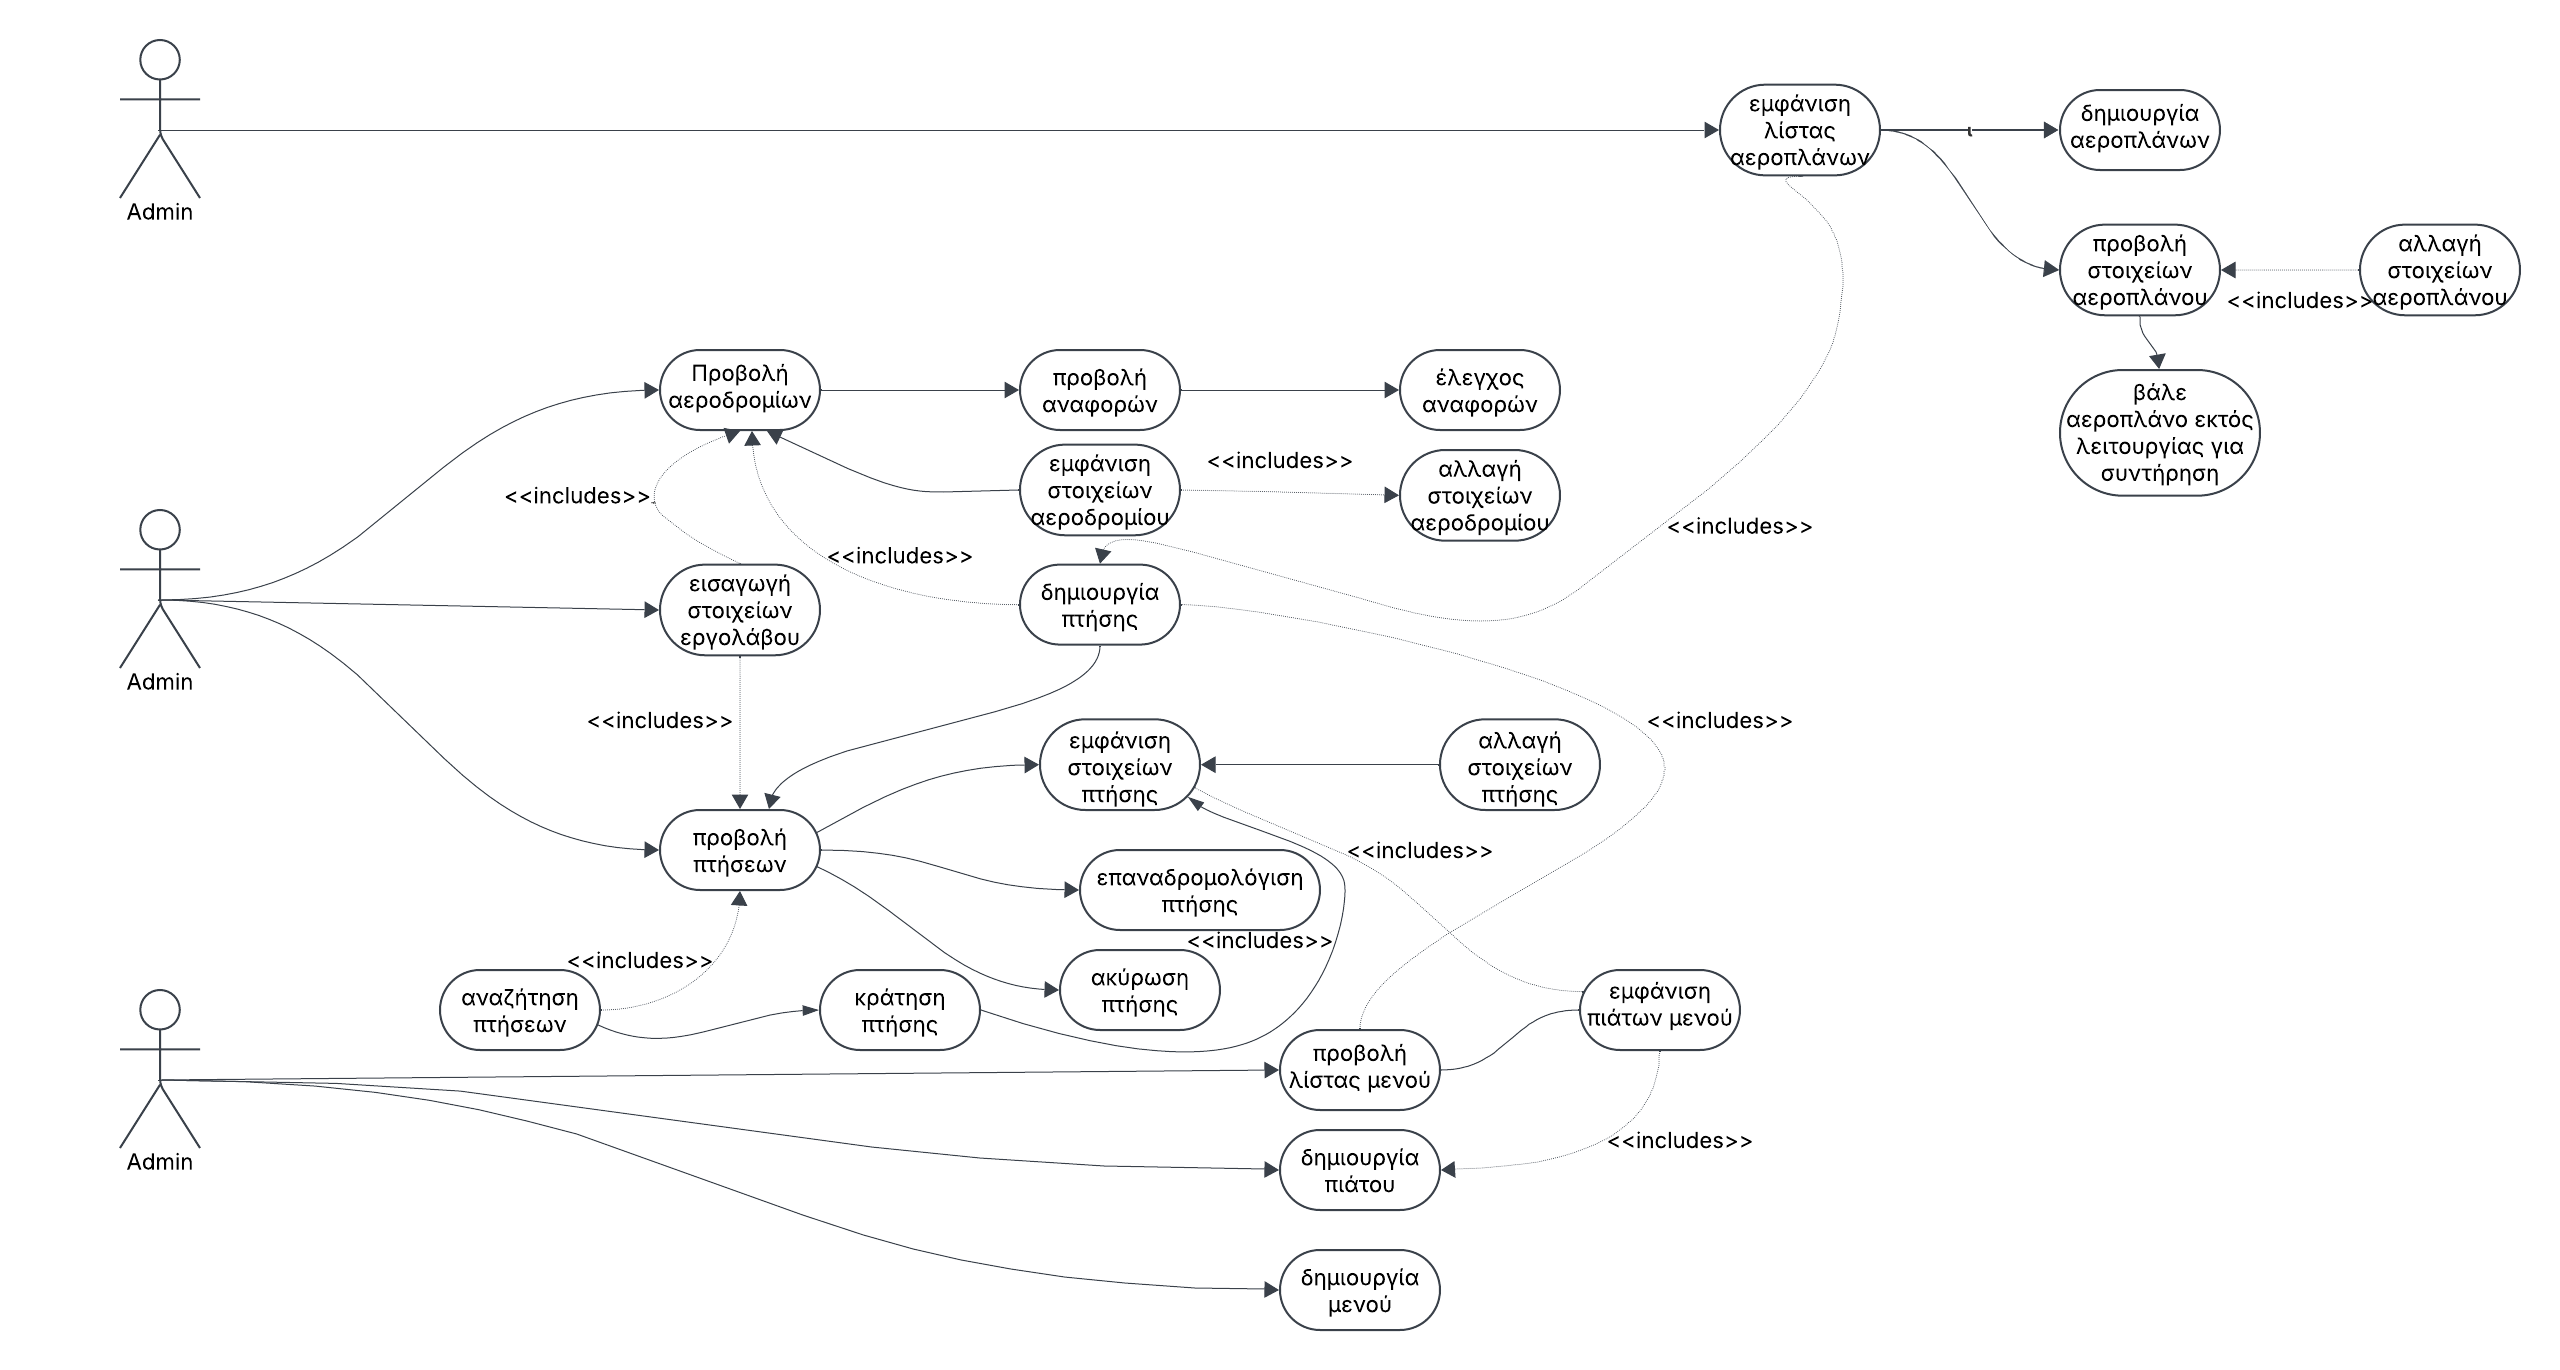
\includegraphics[width=\textwidth]{use-case-diagram.png}
\end{figure}

\section{Προβολή/Προσθήκη Πτήσεων}

% βασική ροή δημιουργίας πτήσης
\basicFlow
\begin{enumerate}
    \item Χρήστης επιλέγει "σχεδίαση πτήσης" \docChange{στην σελίδα προβολής πτήσης}
    \item \docChange{Σύστημα εμφανίζει την σελίδα Σχεδίαση Πτήσης}
    \item\label{uc-step:flight-submit-ready} Χρήστης εισάγει τα στοιχεία της πτήσης που συμπεριλαμβάνει: τον αριθμό πτήσης, αεροδρόμιο αναχώρησης και άφιξης, χρόνους αναχώρησης και άφιξης
    \item\label{uc-step:flight-submitted} Χρήστης πατάει "ολοκλήρωση"
    \item επιστροφή στην κύρια οθόνη
\end{enumerate}

% επιλογή αεροσκάφος
\alternativeFlow
\label{uc-flow:select-airplane-for-flight}
\begin{enumerate}[label=\ref{uc-step:flight-submit-ready}.a.\arabic*]
    \item το σύστημα εμφανίζει στην οθόνη όλα τα αεροπλάνα που μπορούν να εξυπηρετήσουν την πτήση. Δηλαδή να μπορούν να εξηπρετήσουν την πτήση χωρίς να συμπίπτει με τα άλλα δρομολόγια του και να μπορεί να πετάξει στα αεροδρόμια που επέλεξε ο χρήστης.
    \item Χρήστης επιλέγει το αεροπλάνο που θα εξυπηρετήσει την πτήση
    \label{uc-step:plane-selected-for-flight}
\end{enumerate}

% επιλογή αεροσυνοδών
\alternativeFlow
\begin{enumerate}[label=(\ref{uc-step:plane-selected-for-flight}).a.\arabic*]
    \item υπολογίζονται ποιοι αεροσυνοδοί είναι διαθέσιμοι για την πτήση αυτήν συμπεριλαμβάνοντας και τον χρόνο που χρειάζονται για να πάνε από την προηγούμενη πτήση στην επόμενη.
    \item\label{uc-step:creation-of-flight-attendant} Ο χρήστης επιλέγει τους αεροσυνοδούς
    \item επιστροφή στην προηγούμενη ροή
\end{enumerate}

% επιλογή πιλότων
\alternativeFlow
\flowbody{(\ref{uc-step:plane-selected-for-flight}).b.}{
    \item το σύστημα υπολογίζει τους διαθέσιμους πιλότους που θα μπορούν να εξυπηρετήσουν την πτήση αυτήν στην ώρα και τοποθεσία χωρίς να εμποδίζει το προγραμμά τους για προηγούμενες ή επόμενες πτήσεις. Επίσης θα πρέπει να ελέγξει αν οι πιλότοι έχουν την κατάλληλη πιστοποίηση για να πετάξουν το αεροπλάνο και εμφανίζει τους πιλότους στην οθόνη
    \item\label{uc-step:selection-of-pilot-for-flight} ο χρήστης επιλέγει τους πιλότους
    \item επιστροφή στην προηγούμενη ροή
}

% αποθήκευση draft πτήσης
\alternativeFlow
\flowbody{\ref{uc-step:flight-submitted}.a.}{
    \item Δεν έχει επιλέξει ο χρήστης όλα τις απαραίτητες πληροφορίες της πτήσης όπως επιλογή αεροσκάφος, πιλότων και αεροσυνοδών
    \item Χρήστης πατάει υποβολή προσχέδιο πτήσης
    \item αποθηκεύονται οι αλλαγές αλλά η πτήση έχει την ετικέτα προσχέδιο
}

% ακύρωση υποβολής πτήσης
\alternativeFlow
\begin{enumerate}[label=\ref{uc-step:flight-submitted}.b.\arabic*]
    \item Χρήστης επιλέγει "ακύρωση"
    \item το σύστημα διαγράφει όλα τα στοιχεία που μόλις είχε βάλει ο χρήστης για αυτήν την πτήση
\end{enumerate}

% δεν έχουν συμπληρωθεί αρκετά στοιχεία για να δηλωθεί η πτήση
\alternativeFlow
\begin{enumerate}[label=\ref{uc-step:flight-submitted}.c.\arabic*]
    \item δεν έχουν συμπληρωθεί τα απαραίτητα στοιχεία για να δηλωθεί μια μη-εγκεκριμένη πτήση
    \item το submit κουμπί παραμένει απενεργοποιημένο
\end{enumerate}

% έχουν συμπληρωθεί αρκετά στοιχεία μόνο για ένα προσχέδιο πτήσης
\alternativeFlow
\begin{enumerate}[label=\ref{uc-step:flight-submitted}.d.\arabic*]
    \item έχουν συμπληρωθεί τα απαραίτητα στοιχεία για να δηλωθεί μια μη-εγκεκριμένη πτήση αλλά δεν έχουν συμπληρωθεί αρκετά στοιχεία για μια εγκεκριμένη πτήση
    \item Χρήστης πατάει submit
    \item αποθηκεύεται η πτήση με ετικέτα μη-εγκεκριμένη
\end{enumerate}

% έχουν συμπληρωθεί αρκετά στοιχεία για να δηλωθεί μια οριστικοποιημένη πτήση
\alternativeFlow
\begin{enumerate}[label=\ref{uc-step:flight-submitted}.e.\arabic*]
    \item έχουν συμπληρωθεί αρκετά στοιχεία για μια εγκεκριμένη πτήση
    \item Χρήστης πατάει submit
    \item αποθηκεύεται η πτήση με ετικέτα εγκεκριμένη
\end{enumerate}

% ακύρωση πτήσης
\basicFlow
\flowbody{}{
    \item Χρήστης \docChange{επιλέγει} "προβολή πτήσεων" \docChange{στην οθόνη Προβολή Πτήσεων}
    \item\label{uc-step:flight-list} Σύστημα εμφανίζει τις πτήσεις στην οθόνη
    \item\label{uc-step:flight-selected-from-list} Χρήστης επιλέγει πτήση
    \item \docChange{Σύστημα δείχνει την οθόνη προβολή στοιχείων πτήσης}
}

% επιλογή πτήσεων
\alternativeFlow
\flowbody{\ref{uc-step:flight-selected-from-list}.a.}{
    \item Χρήστης \docChange{επιλέγει} προβολή στοιχείων
    \item Σύστημα εμφανίζει όλα τα στοιχεία της πτήσης
    \item Το σύστημα επιτρέπει στον χρήστη να αλλάξει ορισμένα στοιχείας της πτήσεις
    \item\label{uc-step:changing-flight-details} χρήστης κάνει αλλαγές στα πεδία 
    \item Χρήστης επιλέγει υποβολή
}

% φιλτράρισμα πτήσεων
\alternativeFlow
\flowbody{\ref{uc-step:flight-list}.a.}{
    \item χρήστης φιλτράρει πτήση με το αν είναι προσχέδιο ή οριστικοποιημένη
    \item Το σύστημα ενημερώνει την λίστα
    \item επιστροφή στην προηγούμενη ροή
}

% σφάλμα στην επιλογή αεροπλάνουτ
\alternativeFlow
\flowbody{(\ref{uc-step:changing-flight-details}).a.}{
    \item χρήστης έχει επιλέξει αεροπλάνο που έχει λιγότερες θέσεις από αυτό που υπήρχε ήδη
    \item το σύστημα παρουσιάζει μήνυμα σφάλματος και βάζει τον χρήστη να επιλέξει να διαγράψει την πτήση ή να αντιστρέψει την επιλογή αεροπλάνου
    \item χρήστης επιλέγει αντιστροφή επιλογή αεροπλάνου
    \item\label{uc-step:plane-selection-not-allowed} το σύστημα αντιστρέφει την επιλογή αεροπλάνου
    \item επιστροφή στην προηγούμενη ροή
}

\alternativeFlow
\flowbody{(\ref{uc-step:plane-selection-not-allowed}).a.}{
    \item χρήστης επιλέγει διαγραφή πτήσης
    \item ακολουθούμε την ροή βασική ροή που διαγράφει την πτήση
}

\section{Ακύρωση/Επαναδρομολόγηση Πτήσεων}

\bFlowIDReset
\basicFlow
\flowbody{}{
    \item \docChange{Στην οθόνη «Προβολή Πτήσης»} ο χρήστης επιλέγει «ακύρωσης πτήσης»
    \item\label{uc-step:cancelled-flight-plane-rerouting} Σύστημα υπολογίζει αν το αεροπλάνο της πτήσης θα πρέπει να επανατοποθετηθεί για να πραγματοποιηθεί η επόμενη πτήση αν αυτή η πτήση ακυρωθεί.
    \item \docChange{Το σύστημα διαγράφει τους αεροσυνοδούς, πιλότους και το αεροπλάνο από την πτήση}
    \item Το σύστημα διαγράφει ολόκληρη την πτήση \docChange{και εμφανίζει μήνυμα επιτυχίας}
}

\alternativeFlow
\flowbody{\ref{uc-step:cancelled-flight-plane-rerouting}.α.}{
    \item \docChange{Το αεροπλάνο πρέπει να επανατοποθετηθεί}
    \item Σύστημα παρουσιάζει στον χρήστη ένα προειδοποιητικό μήνυμα ότι το αεροπλάνο θα πρέπει να έχει μια πτήσης επανατοποθέτησης για να μπορεί να πραγματοποιηθεί η επόμενη πτήση γιατί αν γίνει η αλλαγή το δρομολόγιο του αεροπλάνου θα έχει κενά και δεν θα μπορεί να τρέχει σωστά ο δρομολογητής μέχρι να φτιαχτεί αυτό το πρόβλημα
    \item Σύστημα βρίσκει αν υπάρχουν πτήσης επανατοποθέτησης που δεν χρειάζονται μεταξύ την πτήσης που ακυρώνεται και την επόμενη πτήση(που δεν είναι πτήση επανατοποθέτησης) και τις ακυρώνει χρησιμοποιώντας την βασική ροή.
    \item \docChange{Χρήστης επιλέγει να συνεχίσει}
    \item Το σύστημα βάζει μια σημαία στην επόμενη πτήση ότι είναι μη-πραγματοποιήσιμη
    \item επιστροφή στην προηγούμενη ροή
}

% reschedule flight
\basicFlow
\flowbody{}{
    \item \docChange{Στην οθόνη προβολής πτήσης} ο χρήστης \docChange{επιλέγει} επαναδρομολόγηση πτήσης
    \item \docChange{Στην οθόνη επαναδρομολόγησης πτήσης} το σύστημα δείχνει μερικές από τις προηγούμενες πτήσης και κάποιες από τις επόμενες πτήσης για να βοηθήσει τον χρήστης για το πότε να επαναδρομογήσει την επόμενη πτήση
    \item Χρήστης επιλέγει να αλλάξει την ώρα της πτήσης
    \item\label{uc-step:rescheduled-flight-changes-required} Σύστημα υπολογίζει αν οι αεροσυνοδοί, πιλότοι και αεροπλάνο θα είναι διαθέσιμοι να λειτουργήσουν την πτήση
    \item\label{uc-step:rescheduled-flight-confirmation} Χρήστης \docChange{επιλέγει} επιβεβαίωση αλλαγών
}

% rescheduled flight needs some changes
\alternativeFlow
\flowbody{\ref{uc-step:rescheduled-flight-changes-required}.α.}{
    \item Αν δεν μπορούν να λειτουργήσουν την πτήση θα τους βγάλει προσωρινά από την πτήση(ακόμα θα είναι αποθηκευμένη στην πτήση στην περίπτωση που πρέπει να αντιστραφούν οι αλλαγές).
    \item Χρήσης επιλέγει με ποιους θέλει να τους αντικαταστήσει και επιλέγει υποβολή
    \item επιστροφή στην βασική ροή
}

% cancel changes to rescheduled flight
\alternativeFlow
\flowbody{\ref{uc-step:rescheduled-flight-confirmation}.α.}{
    \item Χρήστης επιλέγει ακύρωση
    \item Σύστημα αντιστρέφει τις αλλαγές
    \item τερματισμού ροής
}

\alternativeFlow
\flowbody{\ref{uc-step:rescheduled-flight-confirmation}.β.}{
    \item λείπουν πιλότοι, αεροσυνοδοί ή αεροπλάνο από την πτήση
    \item σύστημα απενεργοποιεί το κουμπί "επιβεβαίωση αλλαγών" και άρα ο χρήστης δεν μπορεί να το πατήσει
    \item \docChange{Σύστημα δεν επιτρέπει στον χρήστη να υποβάλει τις αλλαγές και παρουσιάζεται μήνυμα σφάλματος}
    \item επιστροφή στο \textbf{βήμα \ref{uc-step:rescheduled-flight-changes-required}}
}

%menu use case
\section{Διαχείρηση menu}
% βασική ροή δημιουργίας menu
\bFlowIDReset
\basicFlow
\flowbody{}{
    \item\label{uc-step:menu creation} Ο χρήστης επιλέγει το κουμπί "εισαγωγή αντικειμένου menu"
    \item Το σύστημα δημιουργεί το νέο αντικείμενο
    \item Ο χρήστης εισάγει το όνομα, το κόστος και το βάρος του αντικειμένου
    \item\label{uc-step:cancel} Ο χρήστης επιλέγει το πλήκτρο καταχώρηση αντικειμένου
    \item Το σύστημα εισάγει το αντικείμενο στην λίστα των διαθέσιμων αντικειμένων μενού και επιστρέφει στην αρχική οθόνη
}

%εναλλακτική ροή ακύρωση εισαγωγής
\alternativeFlow
\flowbody{\ref{uc-step:cancel}.a.}{
    \item Ο χρήστης επιλέγει το πλήκτρο ακύρωση
    \item Το σύστημα διαγράφει το νέο αντικείμενο και επιστρέφει στην
    αρχική οθόνη
}

%εναλλακτική ροή δημιουργία μενού
\alternativeFlow
\flowbody{\ref{uc-step:menu creation}.a.}{
    \item Ο χρήστης επιλέγει το πλήκτρο δημιουργία μενού
    \item Το σύστημα εμφανίζει την οθόνη δημιουργία μενού και
    φορτώνει τα διαθέσιμα αντικείμενα μενού
    \item Ο χρήστης εισάγει τα στοιχεία του μενού, όνομα και μια μικρή περιγραφή για το ποιές πτήσεις αφορά
    \item Ο χρήστης επιλέγει το αντικείμενο που θέλει να προσθέσει
    στο μενού από τα διαθέσιμα αντικείμενα
    \item\label{uc-step:cancel item} Ο χρήστης επιλέγει το πλήκτρο εισαγωγή αντικειμένου
    \item Το σύστημα αποθηκεύει το αντικείμενο στο μενού. Τα
    βήματα 1.a.4-1.a.6 επαναλαμβάνονται όσο θέλει ο χρήστης
    \item\label{uc-step:cancel menu} Ο χρήστης επιλέγει το πλήκτρο καταχώρηση μενού
    \item Το πρόγραμμα υπολογίζει την τιμή του μενού και το
    συνολικό του βάρος και εμφανίζει μια οθόνη στηνν οποία ο χρήστης μπορεί να αφαιρέσει αντικείμενα και να κάνει την τελική αποθήκευση του menu
    \item το σύστημα αποθηκεύει στην λίστα με τα
    διαθέσιμα μενού. Το σύστημα επιστρέφει στην αρχική
    οθόνη
}

%εναλλακτική ροή ακύρωση εισαγωγής
\alternativeFlow
\flowbody{\ref{uc-step:cancel item}.}{
    \item Ο χρήστης επιλέγει το πλήκτρο ακύρωση
    \item  Το σύστημα ακυρώνει την εισαγωγή του στοιχείου και
επιστρέφει στο βήμα 1.a.4
}

%εναλλακτική ροή ακύρωση μενού
\alternativeFlow
\flowbody{\ref{uc-step:cancel menu}.}{
    \item Ο χρήστης επιλέγει το πλήκτρο ακύρωση μενού
    \item   Το σύστημα διαγράφει όλα τα στοιχεία του μενού και
    επιστρέφει στην αρχική οθόνη
}

\maketitle
\section{Διαχείριση Αναφορών πιλότων}

%βασική ροή αυτόματος έλεγχος αναφορών
\bFlowIDReset
\basicFlow
\flowbody{}{
    \item Το σύστημα παίρνει μια επείγουσα αναφορά από τους πιλότους
    \item Το σύστημα φορτώνει τα στοιχεία της πτήσης από την οποία
    ήρθε η αναφορά και βρίσκει το αεροπλάνο
    \item Το σύστημα ακυρώνει όλες τις προγραμματισμένες πτήσεις με
    αυτό το αεροπλάνο
}

%Βασική ροή χειροκίνητος έλεγχος αναφορών

\basicFlow
\flowbody{}{
    \item Ο χρήστης επιλέγει το πλήκτρο ‘Διαχείριση αναφορών’
    \item Το σύστημα φορτώνει και εμφανίζει μια λίστα με όλα τα
    διαθέσιμα αεροπλάνα
    \item \label{back to main}Ο χρήστης επιλέγει ένα αεροπλάνο
    \item Το σύστημα εμφανίζει και φορτώνει όλες τις πτήσεις που έχουν
    εκτελεστεί με το αεροπλάνο
    \item\label{back to second screen} Ο χρήστης επιλέγει μία πτήση
    \item Το σύστημα φορτώνει και εμφανίζει την αναφορά των πιλότων
    μετά από την πτήση
    \item\label{back to third screen} Ο χρήστης επιλέγει το πλήκτρο ακύρωση πτήσεων
    \item Το πρόγραμμα ακυρώνει όλες τις προγραμματισμένες με αυτό
    το αεροπλάνο πτήσεις
}

%εναλλακτική ροή ακύρωση 1
\alternativeFlow
\flowbody{\ref{back to main}.a.}{
    \item Ο χρήστης επιλέγει το πλήκτρο ‘επιστροφή’
    \item Το σύστημα επιστρέφει στην αρχική οθόνη
}

%εναλλακτική ροή ακύρωση 2
\alternativeFlow
\flowbody{\ref{back to second screen}.a.}{
    \item Ο χρήστης επιλέγει το πλήκτρο επιστροφή
    \item Το σύστημα επιστρέφει στο βήμα 2 της βασικής ροής
}

%εναλλακτική ροή ακύρωση 3
\alternativeFlow
\flowbody{\ref{back to third screen}.a.}{
    \item  Ο χρήστης επιλέγει το πλήκτρο ‘επιστροφή
    \item Το σύστημα επιστρέφει στο βήμα 4 της βασικής ροής
}

%βασική ροή πίνακας αεροδρομίων 
\bFlowIDReset
\basicFlow
\flowbody{}{
    \item Χρήστης επιλέγει τη διαχείριση αεροδρομίων από το σύστημα.
    \item Το σύστημα εμφανίζει λίστα με όλα τα αεροδρόμια που χρησιμοποιεί η αεροπορική εταιρεία.
    \item \label{back to airport list} Χρήστης επιλέγει ένα αεροδρόμιο για προβολή ή επεξεργασία.
    \item Το σύστημα εμφανίζει λεπτομέρειες για το επιλεγμένο αεροδρόμιο, όπως τοποθεσία, χωρητικότητα, ωράριο λειτουργίας, μέγιστος αριθμός πτήσεων, αριθμός διαδρόμων  και μέγιστο μήκος διαδρόμου.
    \item \label{back to airport} Χρήστης μπορεί να τροποποιήσει στοιχεία του αεροδρομίου, όπως ωράριο λειτουργίας ή μέγιστο αριθμό πτήσεων.
    \item Χρήστης επιβεβαιώνει τις αλλαγές.
    \item Το σύστημα αποθηκεύει τις αλλαγές και ενημερώνει τα σχετικά δεδομένα πτήσεων αν χρειάζεται.
}

%εναλλακτική ροή  1
\alternativeFlow
\flowbody{\ref{back to airport list}.a.}{
    \item Ο χρήστης επιλέγει το πλήκτρο ‘επιστροφή’
    \item Το σύστημα επιστρέφει στην αρχική οθόνη
}

%εναλλακτική ροή  2
\alternativeFlow
\flowbody{\ref{back to airport list}.b.}{

    \item Το Χρήστης επιλέγει να προσθέσει νέο αεροδρόμιο.
    \item Το Το σύστημα εμφανίζει φόρμα καταχώρησης νέου αεροδρομίου.
    \item Το Χρήστης συμπληρώνει τα στοιχεία του αεροδρομίου όπως όνομα, μέγιστη χωρητικότητα, αριθμοί διαδρόμων κτλ.
    \item Το Χρήστης πατάει επιβεβαίωση.
    \item Το Το σύστημα καταχωρεί το νέο αεροδρόμιο στη βάση δεδομένων και ενημερώνει τις διαθέσιμες επιλογές δρομολογίων.
}

%εναλλακτική ροή 3
\alternativeFlow
\flowbody{\ref{back to airport}.a.}{

    \item Χρήστης επιλέγει να διαγράψει ένα αεροδρόμιο.
    \item Το σύστημα ελέγχει αν το αεροδρόμιο είναι ενεργό.
    \item Το σύστημα εμφανίζει προειδοποιητικό μήνυμα και δεν επιτρέπει τη διαγραφή σε περίπτωση που είναι ενεργό.
    \item Το σύστημα ζητά επιβεβαίωση από τον χρήστη.
    \item Χρήστης επιβεβαιώνει τη διαγραφή.
    \item Το σύστημα αφαιρεί το αεροδρόμιο από τη βάση δεδομένων.
}


%εναλλακτική ροή  4
\alternativeFlow
\flowbody{\ref{back to airport}.b.}{

    \item Ο χρήστης μπορεί να επισημάνει το αεροδρόμιο ως ανενεργό.
    \item Το σύστημα ενημερώνει αυτόματα όλα τα δρομολόγια που το περιλαμβάνουν και τα χαρακτηρίζει ως μη πραγματοποιήσιμα.
    \item Το σύστημα ειδοποιεί τον διαχειριστή πτήσεων για να αναθέσει εναλλακτικά αεροδρόμια όπου χρειάζεται.
    \item Επιστροφή στη βασική ροή.
}

%εναλλακτική ροή  5
\alternativeFlow
\flowbody{\ref{back to airport}.c.}{
    \item Ο χρήστης επιλέγει το πλήκτρο επιστροφή
    \item Το σύστημα επιστρέφει στο βήμα 2 της βασικής ροής
}


\section{Διαχείριση υπαλλήλων }

%βασική ροή πίνακας υπαλλήλων  
\bFlowIDReset
\basicFlow
\flowbody{}{
    \item Ο χρήστης επιλέγει τη διαχείριση εργαζομένων από το σύστημα.
    \item Το σύστημα εμφανίζει λίστα με όλους τους εργαζομένους της εταιρείας (π.χ., πιλότοι, αεροσυνοδοί, μηχανικοί, διαχειριστές εδάφους).
    \item \label{back to employee list} Ο χρήστης επιλέγει έναν εργαζόμενο για προβολή ή επεξεργασία.
    \item Το σύστημα εμφανίζει λεπτομέρειες του επιλεγμένου εργαζομένου όπως  ID, ηλικία, θέσης εργασίας, ώρες εργασίας κλπ..
    \item \label{back to employee} Ο χρήστης επεξεργάζεται τις πληροφορίες, αν χρειάζεται.
    \item Ο χρήστης επιβεβαιώνει τις αλλαγές.
    \item Το σύστημα αποθηκεύει τις αλλαγές και ενημερώνει τυχόν σχετικές πτήσεις, δρομολόγια ή προγράμματα εργασίας.
}

%βασική ροή πίνακας φίλτρο  
\bFlowIDReset
\basicFlow
\flowbody{}{
    \item Ο χρήστης επιλέγει να προβάλλει διαθέσιμους υπαλλήλους .
    \item Το σύστημα εμφανίζει φίλτρα αναζήτησης, όπως όνομα , ηλικία, δουλειά.
    \item Ο χρήστης επιλέγει τις επιθυμητές παραμέτρους και εκτελεί την αναζήτηση.
    \item Το σύστημα εμφανίζει τη λίστα των διαθέσιμων υπαλλήλους  που ταιριάζουν στα κριτήρια.
    \item Ο χρήστης μπορεί να επιλέξει έναν υπάλληλο για προβολή λεπτομερειών.
    \item Επιστροφή στο μενού διαχείρισης αεροσκαφών.
}

%εναλλακτική ροή 1
\alternativeFlow
\flowbody{\ref{back to employee list}.a.}{
    \item Ο χρήστης επιλέγει το πλήκτρο ‘επιστροφή’
    \item Το σύστημα επιστρέφει στην αρχική οθόνη
}

%εναλλακτική ροή 2
\alternativeFlow
\flowbody{\ref{back to employee list}.b.}{
    \item Ο χρήστης επιλέγει να προσθέσει έναν νέο εργαζομένου.
    \item Το σύστημα εμφανίζει φόρμα εισαγωγής νέου εργαζομένου.
    \item Ο χρήστης συμπληρώνει τα στοιχεία του εργαζομένου
    \item Ο χρήστης επιβεβαιώνει την εισαγωγή.
    \item Το σύστημα καταχωρεί τον νέο εργαζόμενο στη βάση δεδομένων και τον καθιστά διαθέσιμο για μελλοντικές αναθέσεις εργασιών.
}

%εναλλακτική ροή 3
\alternativeFlow
\flowbody{\ref{back to employee}.a.}{
    \item Ο χρήστης επιλέγει να διαγράψει έναν εργαζόμενο.
    \item Το σύστημα ελέγχει αν ο εργαζόμενος είναι ενεργός .
    \item Το σύστημα εμφανίζει προειδοποιητικό μήνυμα και δεν επιτρέπει τη διαγραφή αν ο εργαζόμενος είναι ενεργός.
    \item Αν δεν είναι ενεργός , το σύστημα ζητά επιβεβαίωση από τον χρήστη.
    \item Ο χρήστης επιβεβαιώνει τη διαγραφή.
    \item Το σύστημα αφαιρεί τον εργαζόμενο από τη βάση δεδομένων.
}

%εναλλακτική ροή 4
\alternativeFlow
\flowbody{\ref{back to employee}.b.}{
    \item Ο χρήστης επιλέγει να αλλάξει τους περιορισμούς ενός τύπου εργαζομένου όπως μέγιστες ώρες εργασίας ανά εβδομάδα, απαιτούμενες άδειες.
    \item Το σύστημα ελέγχει αν υπάρχουν εργαζόμενοι που επηρεάζονται από την αλλαγή.
    \item Το σύστημα εμφανίζει ειδοποίηση με τις πιθανές επιπτώσεις όπως ανάγκη για αλλαγές σε βάρδιες ή πτήσεις.
    \item Ο χρήστης επιβεβαιώνει την αλλαγή.
    \item Το σύστημα ενημερώνει τα προγράμματα εργασίας των εργαζομένων που επηρεάζονται.
    \item Επιστροφή στη βασική ροή.
}

%εναλλακτική ροή 5
\alternativeFlow
\flowbody{\ref{back to employee}.c.}{
    \item Ο χρήστης επιλέγει να επισημάνει έναν τύπο εργαζομένου ως μη διαθέσιμο προσωρινά.
    \item Το σύστημα ενημερώνει αυτόματα τα προγράμματα εργασίας και τις πτήσεις, αποδεσμεύοντας προσωρινά τους εργαζομένους αυτού του τύπου.
    \item Αν απαιτείται αντικατάσταση, το σύστημα ειδοποιεί τον διαχειριστή για την ανάγκη εύρεσης εναλλακτικού προσωπικού.
    \item Επιστροφή στη βασική ροή.

}

%εναλλακτική ροή 6
\alternativeFlow
\flowbody{\ref{back to  employee}.d.}{
    \item Ο χρήστης επιλέγει το πλήκτρο επιστροφή
    \item Το σύστημα επιστρέφει στο βήμα 2 της βασικής ροής
}


\section{Διαχείριση αεροπλάνων}

%βασική ροή πίνακας αεροπλάνων 
\bFlowIDReset
\basicFlow
\flowbody{}{
    \item Ο χρήστης επιλέγει τη διαχείριση τύπων αεροσκαφών από το σύστημα.
    \item Το σύστημα εμφανίζει λίστα με όλους τους τύπους αεροσκαφών που χρησιμοποιεί η εταιρεία.
    \item \label{back to airplane list} Ο χρήστης επιλέγει έναν τύπο αεροσκάφους για προβολή ή επεξεργασία.
    \item Το σύστημα εμφανίζει λεπτομέρειες για το επιλεγμένο αεροσκάφος, όπως τύπος αεροσκάφους, χωρητικότητα επιβατών, μέγιστο φορτίο κλπ..
    \item \label{back to airplane} Ο χρήστης επεξεργάζεται τις πληροφορίες αν χρειάζεται.
    \item Ο χρήστης επιβεβαιώνει τις αλλαγές.
    \item Το σύστημα αποθηκεύει τις αλλαγές και ενημερώνει τα σχετικά δεδομένα πτήσεων αν χρειάζεται.
}

%βασική ροή πίνακας φίλτρο  
\bFlowIDReset
\basicFlow
\flowbody{}{ 
    \item Ο χρήστης επιλέγει να προβάλλει διαθέσιμα αεροσκάφη.
    \item Το σύστημα εμφανίζει φίλτρα αναζήτησης, όπως χωρητικότητα επιβατών, εμβέλεια πτήσης, τύπος αεροσκάφους
    \item Ο χρήστης επιλέγει τις επιθυμητές παραμέτρους και εκτελεί την αναζήτηση.
    \item Το σύστημα εμφανίζει τη λίστα των διαθέσιμων αεροσκαφών που ταιριάζουν στα κριτήρια.
    \item Ο χρήστης μπορεί να επιλέξει ένα αεροσκάφος για προβολή λεπτομερειών.
    \item Επιστροφή στο μενού διαχείρισης αεροσκαφών.
}

%εναλλακτική ροή 1
\alternativeFlow
\flowbody{\ref{back to airplane list}.a.}{
    \item Ο χρήστης επιλέγει το πλήκτρο ‘επιστροφή’
    \item Το σύστημα επιστρέφει στην αρχική οθόνη
}


%εναλλακτική ροή 2
\alternativeFlow
\flowbody{\ref{back to airplane list}.b.}{
    \item Ο χρήστης επιλέγει να προσθέσει έναν νέο τύπο αεροσκάφους.
    \item Το σύστημα εμφανίζει φόρμα εισαγωγής νέου τύπου αεροσκάφους.
    \item Ο χρήστης συμπληρώνει τα στοιχεία του αεροσκάφους (τύπος, χωρητικότητα, μέγιστο φορτίο, εμβέλεια κτλ.).
    \item Ο χρήστης επιβεβαιώνει την εισαγωγή.
    \item Το σύστημα καταχωρεί το νέο αεροσκάφος στη βάση δεδομένων και το καθιστά διαθέσιμο για μελλοντικά δρομολόγια.
}

%εναλλακτική ροή 3
\alternativeFlow
\flowbody{\ref{back to airplane}.a.}{
   \item Ο χρήστης επιλέγει να διαγράψει έναν τύπο αεροσκάφους.
   \item Το σύστημα ελέγχει αν το αεροσκάφος είναι ενεργό.
   \item Το σύστημα εμφανίζει προειδοποιητικό μήνυμα και δεν επιτρέπει τη διαγραφή αν είναι ενεργό.
   \item Το σύστημα ζητά επιβεβαίωση από τον χρήστη.
   \item Ο χρήστης επιβεβαιώνει τη διαγραφή.
   \item Το σύστημα αφαιρεί το αεροσκάφος από τη βάση δεδομένων.
}


%εναλλακτική ροή 4
\alternativeFlow
\flowbody{\ref{back to airplane}.b.}{
   \item Ο χρήστης μπορεί να επισημάνει ένα αεροσκάφος ως ανενεργό.
   \item Το σύστημα ενημερώνει αυτόματα όλα τα δρομολόγια που το περιλαμβάνουν και τα χαρακτηρίζει ως μη πραγματοποιήσιμα.
   \item Το σύστημα ειδοποιεί τον διαχειριστή πτήσεων να αναθέσει εναλλακτικά αεροσκάφη όπου χρειάζεται.
   \item Επιστροφή στη βασική ροή.
}

%εναλλακτική ροή 5
\alternativeFlow
\flowbody{\ref{back to  airplane}.c.}{
    \item Ο χρήστης επιλέγει το πλήκτρο επιστροφή
    \item Το σύστημα επιστρέφει στο βήμα 2 της βασικής ροής
}

%Βασική ροή Ανάθεση Εργολάβων στο Αεροδρόμιο 

\section{Ανάθεση εργασίας σε εργολάβους}
\bFlowIDReset
\basicFlow
\flowbody{}{
    \item Ο διαχειριστής επιλέγει το πλήκτρο "ανάθεση εργασίας σε εργολάβο"
    \item Το σύστημα φορτώνει την σελίδα εισαγωγής πληροφοριών για την εργασία
    \item Ο διαχειριστής εισάγει τα στοιχεία της εργασίας που θέλει να γίνει
    \item\label{cancel page 1} Ο χρήστης επιλέγει το πλήκτρο "continue" και το σύστημα φορτώνει τους διαθέσιμους εργολάβους για εκείνο το αεροδρόμιο με πληροφορίες για την δουλειά και την χρέωσή τους.
    \item\label{cancel page 2} Ο χρήστης επιλέγει εργολάβο
    \item Το σύστημα φορτώνει μια σελίδα με όλες τις πληροφορίες για την εργασία και τις πληροφορίες του εργολάβου που έχει επιλεγεί
    \item \label{cancel page 3} Ο διαχειριστής εγκρίνει την συνεργασία 
    \item Το σύστημα καταχωρεί την συνεργασία

}

% Επιστροφή οθόνη 1
\alternativeFlow
\flowbody{\ref{cancel page 1}.a.}{
    \item Ο χρήστης επιλέγει το πλήκτρο επιστροφή
    \item Το σύστημα επιστρέφει στην αρχική οθόνη
}

%Επιστροφή οθόνη 2
\alternativeFlow
\flowbody{\ref{cancel page 2}.a.}{
    \item Ο χρήστης επιλέγει το πλήκτρο επιστροφή
    \item Το σύστημα επιστρέφει στην προηγούμενη οθόνη
}

%Εμφάνιση ενεργών συνεργασιών
\alternativeFlow
\flowbody{\ref{cancel page 2}.b.}{
    \item Ο χρήστης επιλέγει το πλήκτρο εμφάνιση contructs
    \item Το σύστημα φορτώνει την σελίδα με τα cintructs που τρέχουν
    \item Ο χρήστης επιλέγει μια συνεργασία και επιλέγει την ολοκλήρωσή της
    \item Το σύστημα φορτώνει μια οθόνη ολοκλήρωσης και ο χρήστης επιλέγει την πληρωμή του contruct
}

%Επιστροφή οθόνη 3
\alternativeFlow
\flowbody{\ref{cancel page 3}.a.}{
    \item Ο χρήστης επιλέγει το πλήκτρο επιστροφή
    \item Το σύστημα επιστρέφει στην προηγούμενη οθόνη 
}
% Αναζήτηση Πτήσης
\section{Αναζήτηση πτήσης}
\bFlowIDReset
\basicFlow
\flowbody{}{
    \item Ο χρήστης επιλέγει την ενότητα "Αναζήτηση Πτήσης"
    \item Το σύστημα εμφανίζει διαθέσιμες πτήσεις με ώρα, τιμή, αριθμό πτήσης και συνοπτική περιγραφή.
    \item\label{uc-step:user buys} Ο χρήστης επιλέγει πτήση πατώντας το κουμπί «Αγορά».
    \item Το σύστημα εμφανίζει περίληψη πτήσης και πεδία εισαγωγής στοιχείων επιβατών.
    \item\label{uc-step:fill-passenger-data} Ο χρήστης συμπληρώνει για κάθε επιβάτη: Όνομα, Επώνυμο, Email, Ημερομηνία Γέννησης, Αρ. Διαβατηρίου.
    \item Ο χρήστης επιλέγει αν επιθυμεί επιπλέον υπηρεσίες (π.χ. priority boarding).
    \item Το σύστημα υπολογίζει και εμφανίζει την τελική τιμή κράτησης.
    \item Ο χρήστης πατάει «Οριστικοποίηση Κράτησης».
    \item Το σύστημα αποθηκεύει την κράτηση και εμφανίζει μήνυμα επιβεβαίωσης.
    \item\label{uc-step:email sent to passenger} Το σύστημα αποστέλλει email επιβεβαίωσης πτήσης σε κάθε επιβάτη.
    \item Σημείωση εμφανίζεται στην οθόνη: «Η πληρωμή πραγματοποιείται από τον gate agent πριν την επιβίβαση.»
}

\alternativeFlow
\flowbody{\ref{uc-step:user buys}.a.}{
    \item Ο χρήστης προσπαθεί να επιλέξει πτήση που μόλις έγινε sold out.
    \item Το σύστημα εμφανίζει μήνυμα «Η πτήση δεν είναι πλέον διαθέσιμη».
    \item Ο χρήστης επιλέγει άλλη πτήση και η ροή συνεχίζεται από το βήμα 3.
}

\alternativeFlow
\flowbody{\ref{uc-step:fill-passenger-data}.a.}{
    \item Ο χρήστης αφήνει κενά πεδία σε στοιχεία επιβάτη.
    \item Το σύστημα επισημαίνει τα υποχρεωτικά πεδία και μπλοκάρει την ολοκλήρωση.
    \item Ο χρήστης τα συμπληρώνει και η ροή συνεχίζεται από το βήμα 6.
}

\alternativeFlow
\flowbody{\ref{uc-step:email sent to passenger}.a.}{
    \item Η αποστολή email αποτυγχάνει προσωρινά.
    \item Το σύστημα αποθηκεύει κανονικά την κράτηση και εμφανίζει μήνυμα «Η αποστολή email θα επαναληφθεί».
    \item Η ροή συνεχίζεται από το βήμα 11.
}		

% Συντήρηση Αεροσκαφών
\section{Συντήρηση αεροσκαφών}
\bFlowIDReset
\basicFlow
\flowbody{}{
    \item Επιλέγει την ενότητα "Συντήρηση Αεροσκαφών"
    \item\label{uc-step:display plane list} Το σύστημα εμφανίζει λίστα με τα μη διαθέσιμα αεροσκάφη.
    \item Ο διαχειριστής επιλέγει αεροσκάφος.
    \item\label{uc-step:show future flights} Εμφανίζονται οι μελλοντικές πτήσεις του και η αναφορά με την οποια το αεροσκάφος μπήκε ανενεργό.
    \item\label{uc-step:maintenance date} Ο διαχειριστής ορίζει ημερομηνίες συντήρησης.
    \item Αν δεν υπάρχουν συγκρούσεις, εμφανίζεται προεπισκόπηση προγραμματισμού.
    \item\label{uc-step:confirm maintenance} Ο διαχειριστής επιβεβαιώνει την καταχώρηση.
    \item Το σύστημα εμφανίζει ενημέρωση: «Η συντήρηση καταχωρήθηκε επιτυχώς.»
}

\alternativeFlow
\flowbody{\ref{uc-step:display plane list}.a.}{
    \item Δεν υπάρχουν διαθέσιμα αεροσκάφη.
    \item Εμφανίζεται μήνυμα και η διαδικασία ακυρώνεται.
}

\alternativeFlow
\flowbody{\ref{uc-step:show future flights}.a.}{
    \item Το επιλεγμένο αεροσκάφος δεν έχει προγραμματισμένες πτήσεις.
    \item Ο διαχειριστής συνεχίζει κανονικά με την καταχώρηση.
}

\alternativeFlow
\flowbody{\ref{uc-step:maintenance date}.a.}{
    \item Η ημερομηνία έναρξης συντήρησης είναι μετά τη λήξη.
    \item Το σύστημα εμφανίζει προειδοποίηση και ζητά διόρθωση.
}

\alternativeFlow
\flowbody{\ref{uc-step:confirm maintenance}.a.}{
    \item Ο διαχειριστής ακυρώνει πριν επιβεβαιώσει.
    \item Η διαδικασία ακυρώνεται χωρίς καταχώρηση.
}

\end{document}
